\documentclass[twocolumn]{preport}
\usepackage[dvipdfmx]{graphicx}
\graphicspath{{figs/}}
\setlength\abovecaptionskip{0pt}
\setlength\intextsep{5pt}

\title{2018年中間試問要旨:\\
等身大ヒューマノイドにおける三次元環境認識に基づく自律歩行計画に関する研究}
\author{稲葉・岡田研究室  指導教員 稲葉雅幸 教授\\
  機械情報工学科4年 03-160274 大森 悠貴 }

\begin{document}

\pagestyle{empty}
\maketitle
\thispagestyle{empty}
\sloppy

\section{はじめに}
%% 研究背景・課題・手法
%% 近年,災害現場などの人間が立ち入ることが難しい現場において,ロボットが代わりに作業を行うことが期待され,それに伴い災害現場で活躍するロボットの研究が盛んになってきている.
%% 特に等身大ヒューマノイドは,人間と同程度のサイズ,自由度を持ち,車輪だけでは立ち入れない場所へ立ち入ったり,人間が行うことのできる多くのタスクを実現することが期待されている
%% 2015年にアメリカで行われた,DARPA ROBOTICS CHALLENGEでは,災害現場を模した環境で複数のタスクが課せられ,それに取り組む中で様々な課題が浮き彫りになった.

%% その一つとして,不整地における自律的な歩行計画が挙げられる.(修正する)
%% 一点目に,認識に基づく着地位置の検出の問題がある.
%% 現状,足の着地位置としては,足平の四頂点と中心に点群があるかどうかで判定されている(あやしい).
%% この手法では,完全平面を前提とした着地位置のみしか着地可能箇所として認識されず,実際の災害現場などで使うことは難しい.
%% (あきらかに着地不可能な場所を着地可能としてしまう問題がある)

%% 本研究では,

近年,災害現場などで人間の代わりにロボットが作業を行うことが期待されている.
特に等身大ヒューマノイドは,台車型ロボットでは難しい多様な足場環境でも立ち入れる機構を有しており,人間中心環境で様々な作業に対応することができると考えられる.
しかし,現状多くのヒューマノイドは固定された足場,平面を前提とした歩行計画を行っており,そうした多様な足場での歩行を実現できていない.
また,不安定な足場を含む場合,視覚による認識だけでは安定的に目標地までたどり着くには不十分である.
これらを踏まえ,本研究では視覚,触覚,記憶に基づく多様な足場環境への対応できるシステムの確立に取り組む.
%% これらを踏まえ,本研究では視覚情報に基づき平面以外の足場候補を拡大すること,足裏の触覚情報に基づき足場の安定性を確認することにより,複雑な足場環境で安定的に目標地に到達するシステムの確立に取り組む.


\section{多様な足場環境に対応する自律歩行計画}

はじめに,足平の支持領域と接触領域の関係,安定性,幾何学的特徴により足場の分類を行ったものを\figref{category}に示す.
このうち,一番左上の領域は,多くのヒューマノイドロボットが歩行計画をする際に用いる足場である.
上段の左から二番目の領域はWiedebachら\cite{wiedebach2016walking}により,上半身のバランスをとることで実現されている.
%% また,窪んだ足場や球面の点着地についても,\cite{kanoulas2017vision}により,曲面パッチを用いることで実現されている.
これらに加え,支持領域と接触領域がことなる足場を認識により着地位置候補に含め,下段の動的な足場を足探りによる安定性を確認した上で着地候補に含めることで,複雑な足場環境でも十分に着地可能な足場を確保できると考えられる.

%% パワポの分類図
\begin{figure}[tbh]
 \begin{center}
   \centering
   \includegraphics[width=0.87\columnwidth]{category.pdf}
   \caption{着地可能足場の分類}
   \label{figure:category}
 \end{center}
\end{figure}

次に,この分類を踏まえた視覚,触覚を用いた,多様な足場環境に対応するシステムを\figref{system}に示す.
%% 毎回足場の確認をするのは時間的コストがかかるため,記憶に基づく安全確認の省略により目的地到達時間の短縮を図る
効率化のため,記憶に基づく安全判断も合わせて行う.

%% システム構成図
\begin{figure}[tbh]
 \begin{center}
   \centering
   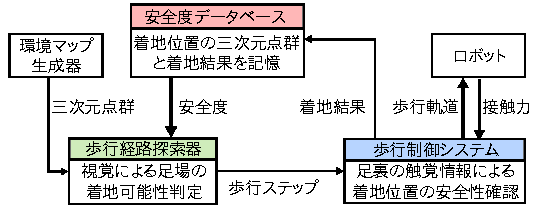
\includegraphics[width=\columnwidth]{system_fig.pdf}
   \caption{システム構成図}
   \label{figure:system}
 \end{center}
\end{figure}

\subsection{視覚情報に基づく着地可能候補の拡大}
植田ら\cite{ueda2015dron}の手法に基づきハードウェアの制約から可能な領域を離散的な足配置で近似し,離散グラフの最良優先探索により歩行計画を行う.
三次元環境点群情報に足配置を射影し,点群上に足配置が可能かどうかを判定する.その際に,従来の平面だけでなく,離散的な足場でも足平を安定して着地させることが可能であれば,着地の可能判定を出せるように改良する.また,支持領域に基づき,ZMPの位置を一ステップごとに修正し,安定した着地を可能にする.

\subsection{触覚情報に基づく足場安定性の確認}
ZMPを支持脚の支持領域に収めたまま,遊脚による次のステップの足場の安定性を,少しだけ踏み込むことによって確認する.
足裏の力センサを使用し,認識の高さ方向の情報を用いた推定圧力とセンサ値を比較し,足場として着地可能かを判断する.
着地不可能と判断した場合は,その足場を使わない歩行経路を再計算する.

\subsection{記憶情報に基づく足場安全性の見積}
また,足場の安定性が確認されたものについては,視覚情報と合わせて記憶することで,次回以降同様の足場への着地をする際に,足場の安定性確認を省くことによる目標到達時間の短縮を試みる.


\section{踏みしめによる足場環境確認実験}
等身大ヒューマノイドと同じ脚をもつ二脚ロボットを用いて,遊脚による足場の安定性を確認する実験を行った.
安定な足場と不安定な足場を踏んだ時の力センサの値の変化のグラフを\figref{exp}示す.
静的足場として板を,動的足場として柔らかいマットを用いた.
実験は複数回行ったが,足場により接触力遷移に差が確認できた.

\begin{figure}[tbh]
 \begin{center}
   \centering
   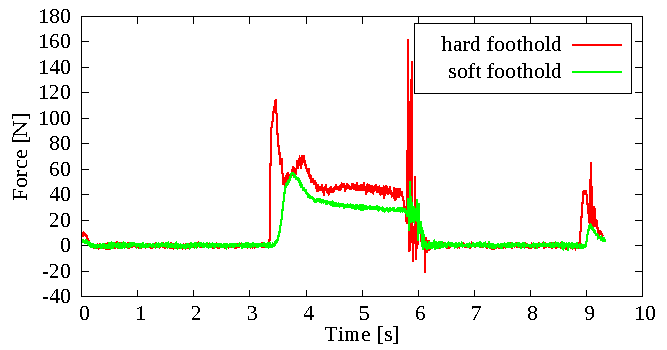
\includegraphics[width=0.8\columnwidth]{exp_foothold_check.pdf}
   \caption{踏みしめによる足裏の接触力遷移}
   \label{figure:exp}
 \end{center}
\end{figure}

%% このあたりに考察を書く


\section{おわりに}
% 全体をまとめる
%% 本研究では,視覚・触覚・記憶を用いることにより,多様な足場環境下で歩行を可能にする個々のモジュールと全体システムを考案した.
%% 今後は,提案手法を実装し,多様な足場への着地を試みる他,具体的なデータベースの構造設計を行う.

今後は2章で提案した手法を実装し,シミュレーション・実機による歩行実験を行う.
また,踏みしめによる安定性確認の追加実験,具体的なデータベースの構造設計を行う.
これらを踏まえて,不整地歩行システムの確立を目指す.



\small
\bibliographystyle{junsrt}
\bibliography{p-report}


\end{document}



%% 2017中間試問
%% 動的な環境で人間とロボットが共に過ごすためには,認識や行動の高速化が求められる.
%% しかし,動的な環境では正確な認識が難しい,またシミュレータ上で完全なロボットモデルが作成できないことから,ダイナミックな動きをするとシミュレータと実際の環境との差異が生じてしまう.
%% そのため,実際の環境の不確実な情報からでも,適切な動作生成ができるようになることが必要である.

%% 高速な動作生成をしている先行研究として,T. Senooらの高速バッティングの研究\cite{Ishikawa}があるが,環境固定のカメラを用いており,スタンドアローンに動作するヒューマノイドには適用できない.
%% またR. Terasawaらの高速スイング\cite{Terasawa}はオフラインで軌道を生成したものを再生しており,認識に基づいた動作生成ができていない.

%% 本研究では,素早い認識と動作生成が求められる行動として,テニスのボレー動作を題材とする.

%% ゴミ
%% これらの素早い認識,行動が特に求められるのは主に動的環境下においてである.
%% このような動作を実現するため,比較的速い動作が可能なヒューマノイドロボットであるJAXON\cite{Kojima}を用いて研究を行う.
%% 将来的にヒューマノイドロボットが日常生活環境で動作する際,すぐにその環境に馴染んで本来持つパフォーマンスができることが望ましい.特定の環境下でしか動作できないのは望ましくない.
%% 現状,ある環境にロボットを適応させるには,その環境でのチューニングをしなければならないことが多い.
%% また日常生活環境は常に変化する環境である.こうした外界の状況を把握するためにも

%% ゴミ
%% \section{ボレー動作実現へのアプローチ}
%% 不確実なボールの座標情報から軌道を予測する方法として,単純な物理モデルを考慮した手法,つまりは回帰曲線を利用した軌道の直線近似や放物線近似がある.このモデルが有効なのは,ノイズが軌道に対して正規分布している状況であり,ノイズに何かしらの偏りがあるとうまく軌道を推定することができない.当然これらのノイズの原因がわかればそれに沿ったモデルを適用することにより推定が正しく行えるが,そうでない場合も多い.そこで,学習という手法を用いることで,ノイズをうまく吸収できるのではないかと思われる.
%% \subsection{既知の認識と動作生成の高速化}
%% ボールの座標情報から軌道を予測する方法として,運動モデルに基づいて軌道予測する手法がある.
%% このモデルの精度を上げるためには,どのようなノイズが乗るかを想定する必要があるが,ノイズをすべて想定するのは難しい.
%% そこで,学習を用いることで,想定外のノイズにも対応することを考える.
%% ノイズが乗るのが認識だけであれば軌道予測だけに学習を用い,動作生成は最適計算により行えば良いが,高速な動作生成もシミュレータの計算結果と差異を生じるため,動作生成も含めた学習器を考える.

%% 2017中間試問
%% ボレー動作をする一つのアプローチとして運動モデルに基づいて軌道予測をし,目標位置に対して逆運動学を計算する手法が考えられる.
%% 所望の動作を実環境で実現するためには運動モデルを正しく見積もる必要がある.
%% しかし,実環境では多様な外乱が存在するために運動モデルに基づいた正確な軌道予測と動作実現が難しい.
%% そのため,運動モデルを必要としない学習を用いた認識と動作生成のアプローチを本研究では考える.
%% 学習を用いた認識と動作生成のシステム構成図を\figref{system}に示す.
%% まず,カメラのRGB画像を画像処理した後,対象物体の三次元座標を計算する.
%% そして,動作生成直前までの三次元座標時系列データを入力として
%% ボレー動作を生成するような学習器を設計する.
%% 動作生成については,目標設定後にボレーの動作のための逆運動学計算をするのでは間に合わないと考えられるため,
%% 予め基本動作となる高速なボレー動作をデータベースの中に複数用意しておく.
%% 学習器によりデータベースから適切な基本動作を選択し,タイミングと打点位置修正値を与えることでボレー動作を実現する.
%% データベースに,呼び出す基本動作,基本動作でカバーできない範囲のボールに対応するための打点位置調整パラメータ,打球タイミングを与えることにより,非常に少ない計算量で動作生成を実現することが可能になる.
%% 更に実環境での外乱を補償するために,実際の行動結果を評価して学習器のパラメータを更新する.
%% 評価はボールが相手コート内に返せているかどうか,飛んできた方向に打ち返せているかどうか決定する.


%% \subsection{認識から高速動作を呼び出すための}
%% これらを組み合わせたシステム構成図を\figref{system}に示す.
%% ボール軌道の推定は中間層に含まれているものとし,入力はボールの三次元座標の時系列データ,出力はデータベースから呼び出すモーション番号,モーションを微調整するための誤差修正パラメータ,再生するタイミングとして学習器を設計する.評価はボールが相手コートないに返せているかどうか,飛んできた方向に打ち返せているかどうか決定する.
%% 認識と動作生成を組み合わせたシステム構成図を\figref{system}に示す.
%% ボールの軌道予測,打点の目標位置は明示的に出力せず,認識を入力,動作生成を出力としたend-to-endな動作生成器を作成する.
%% 入力はボールの三次元座標の時系列データ,出力は基本動作選択,打点位置調整,打球タイミングとして学習器を設計する.
%% 評価はボールが相手コート内に返せているかどうか,飛んできた方向に打ち返せているかどうか決定する.




%% 事前学習としてテストデータを用いた教師付き学習を行い,その後実機による強化学習を行う.
%% これらを組み合わせることによりボレーの動作の実現を目指すが,ボール軌道の推定は中間層に含まれているものとし,入力はボールの三次元座標の時系列データ,出力はデータベースから呼び出すモーション番号,モーションを微調整するための誤差修正パラメータ,再生するタイミングという学習器を設計する.評価はボールが相手コートないに返せているかどうか,飛んできた方向に打ち返せているかどうか決定する.


%% 2017中巻試問
%% \begin{figure}[tbh]
%%  \begin{center}
%%    \centering
%%    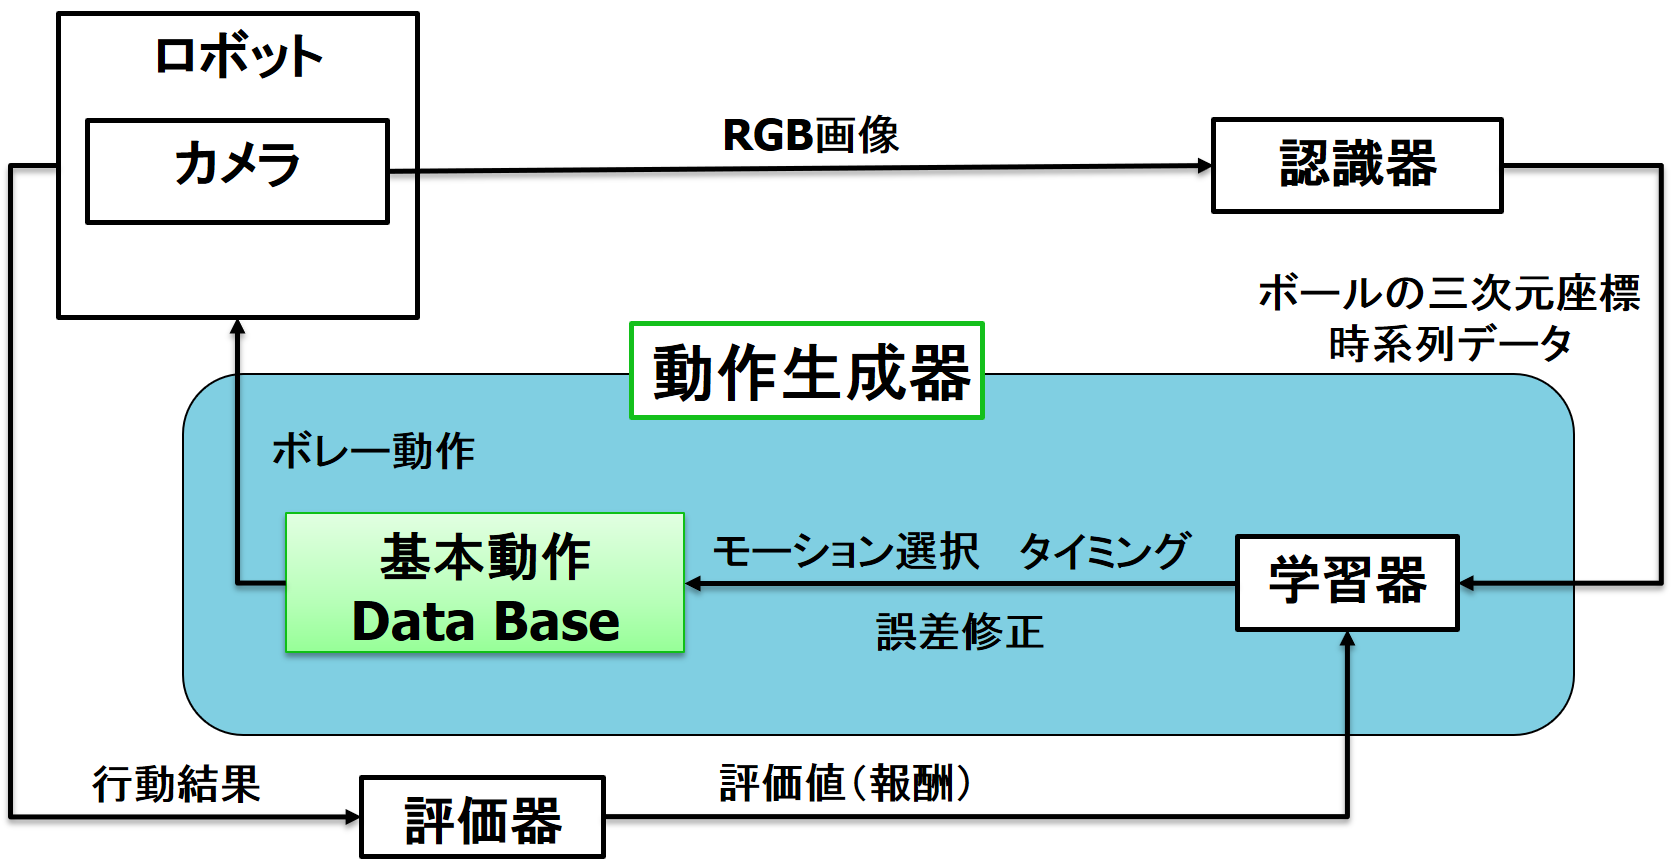
\includegraphics[width=\columnwidth]{system_fig.png}
%%    \caption{システム構成図}
%%    \label{figure:system}
%%   %% \hspace{0.02\columnwidth}
%%   %% \begin{minipage}{0.32\columnwidth}
%%   %%   \centering
%%   %%  \includegraphics[width=0.7\columnwidth]{jaxon2_appearance.png}
%%   %%  \caption{JAXON\cite{Kojima}}
%%   %%  \label{figure:est_graph}
%%   %% \end{minipage}
%%  \end{center}
%% \end{figure}


%% 2017中巻試問
%% \section{検証実験}
%% 学習を用いたシステムを導入するための検証実験として,
%% 現状の認識・軌道予測の精度,動作生成にかかる時間を把握するための実験を行った.

%% \subsection{実際のボール投球による認識と軌道予測実験}
%% ボールの三次元座標がどの程度のノイズを含んだ不確実な情報になっているかを確かめるため,実際にボールを投げ,各時刻のボールの三次元座標を両眼視差により計算するとともに,線形回帰によりどの程度正確に軌道予測,打点推定が行えるのかを調べた.

%% \figref{coords_graph}はボールの三次元座標の時間変化を示したグラフである.
%% いずれの座標のグラフにおいても振動的であり,特に奥行き方向の座標の振動が大きいことがわかる.
%% \figref{est_graph}は\figref{coords_graph}の時間変化を用い,カメラから1m先の奥行き方向に対して垂直な平面上のどの座標にボールが来るかを予測したものである.\figref{est_graph}上段がx,z座標の時間変化から計算した水平方向の座標であるが0.3mの幅で振動しており,下段がx,y,z座標の時間変化から計算した鉛直方向の座標であるが,振動幅10mと予測に使うのは難しい.

%% \begin{figure}[tbh]
%%  \begin{center}
%%   \begin{minipage}{0.6\columnwidth}
%%    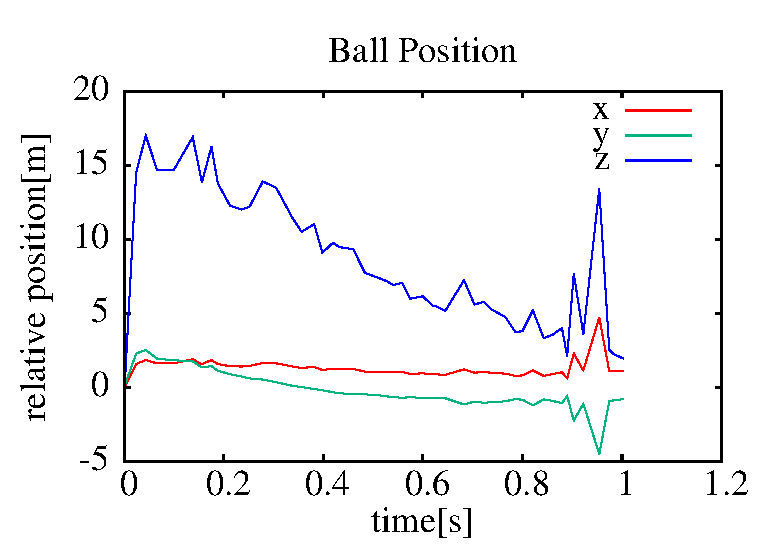
\includegraphics[width=\columnwidth]{ball_coords_316.eps}
%%    \caption{座標の時間変化}
%%    \label{figure:coords_graph}
%%   \end{minipage}
%%   %% \hspace{0.05\columnwidth}
%%   \begin{minipage}{0.35\columnwidth}
%%    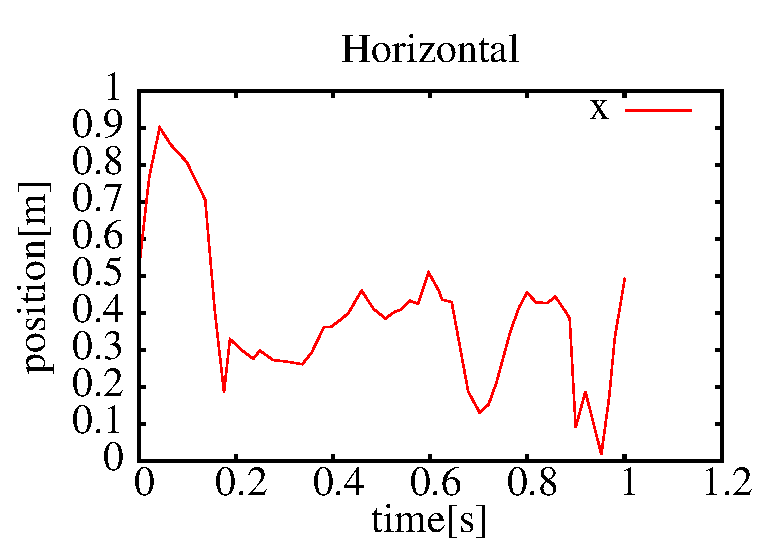
\includegraphics[width=\columnwidth]{est_x_316.eps}
%%    %% \caption{軌道予測}
%%    %% \label{figure:est_x_graph}
%%   %% \end{minipage}
%%   %% \begin{minipage}{0.3\columnwidth}
%%    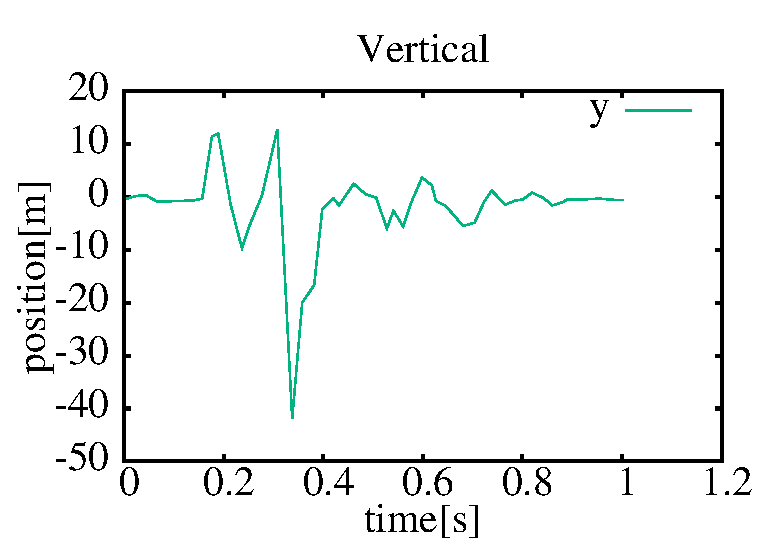
\includegraphics[width=\columnwidth]{est_y_316.eps}
%%    \caption{打点推定}
%%    \label{figure:est_graph}
%%   \end{minipage}
%%  \end{center}
%% \end{figure}

%% 2017中間試問
%% \subsection{ボール位置にラケットを差し出す動作生成実験}
%% ラケットをロボットから奥行き方向に1m先で固定し,ボールと同じ鉛直水平座標を目標として差し出す実験を行い,動作生成にかかる時間や生成される動作について確かめた.

%% 逆運動学を解き直す必要がある際に時間がかかることや,ラケットを目標位置に持ってくるだけでなく,打点までのラケットの軌道も考慮する必要があることが確認できた.
%% 連続してikを解くと腕がねじれてしまうため,毎回初期姿勢からikを解きなおす必要があることがわかった.また,関節角度に応じて移動速度を決めているため,初期姿勢をできるだけボレー動作に近いものにしたほうが良いことや,ラケットの軌道を考える必要があることがわかった.


%% \section{おわりに}
%% %% 検証実験により,認識や動作生成の課題が浮き彫りになった.
%% %% 今後は2章で提案した学習を用いるアプローチに基づき,使用する学習モデルの決定し,教師付き学習による事前学習を行った上で実機での強化学習を行う.
%% %% 学習によって未知のノイズを吸収するとしても,奥行きが少しでも正確な値が出る方が学習に時間がかからないため,Depthセンサを取り付けたり,ボールの画面上での大きさの情報を用いることによる解決を目指す.
%% %% 同時に微調整が可能なボレーモーションを作成し,調整可能範囲を検証する.
%% %% 最終目標としては人とボレーのラリーをできるレベルまで持って行きたい.
%% %% 事前学習としてテストデータを用いた教師付き学習を行い,その後実機による強化学習を行う.
%% 今後は2章で提案した学習を用いるアプローチに基づき,使用する学習モデルを決定し,教師付き学習による事前学習を行った上で実機での強化学習を行う.
%% 同時に微調整が可能なボレーモーションを作成し,調整可能範囲を検証する.
%% 最終目標としては人とのラリーの実現を目指す.
